\apendice{Documentación de usuario}

\section{Introducción}
Esta sección recoge las instrucciones y conocimientos técnicos que un usuario debe conocer para poder utilizar el laboratorio presentado. \\
Veremos cómo instalar el software en nuestra placa y cómo controlar la placa maestro. Se explicarán las funciones que realiza cada botón y cuáles son los usos que tiene el laboratorio.

\section{Requisitos de usuarios}

Para poder utilizar el programa lo primero es disponer de todas las piezas que componen el laboratorio.
Deberemos comprobar que todos los componentes están correctamente conectados entre sí. Para ello deberemos:
\begin{enumerate}
\item Disponer de tres cables ethernet con clavija RJ-45 y conectar cada uno de ellos a una placa y a un switch.
\item Comprobar que los motores están correctamente conectados a la placa controladora y que las placas FRDM k64F también están conectadas a la placa controladora de los motores. Es importante cerciorarnos de que todos los pines están debidamente conectados a su posición  correspondiente. 
\item Tendremos que asegurarnos que todos los componentes están conectados a una toma de corriente y reciben energía, por lo general si están recibiendo corriente tendrán algún led encendido.
\item También deberemos comprobar que el switch cumple con su función mirando si todos los puertos donde se conectan los cables de red están recibiendo y enviando datos.
\item Se deberá conectar la placa de expansión a la placa maestro, en este caso es muy sencillo porque solo existe una forma de conectarla para que todos los pines queden conectados.
\item Por último deberemos conectar los pines de la pantalla LCD a una de las placas maestro para poder ver de manera adecuada la información de los comandos recibidos.
\end{enumerate}

Para la conexión de los pines de los motores y la pantalla se puede consultar el apéndice anterior, concretamente la sección \ref{distribucionDePines}
Tras tener configurado el entorno, el siguiente paso será cargar el programa correspondiente a cada microcontrolador. Recordemos que disponemos de tres placas y tres \extranjerismo{softwares} con algunas diferencias entre ellos. En el apéndice anterior \ref{sec:compilacion} ya vimos como podíamos realizar este procedimiento.
Una vez se tienen los códigos cargados en las placas deberemos, esperar a que los tres microcontroladores adquieran su respectiva dirección IP y podremos comenzar a enviar comandos desde la placa maestro como veremos en el siguiente apartado.

\section{Manual del usuario}
En el apéndice 3 \ref{Ap:requisitos} pudimos ver en los requisitos funcionales todos los usos de la placa y sus correspondientes pasos. En este apartado veremos de una forma más gráfica las utilidades de la misma.

En primer lugar vamos a visualizar y nombrar los botones de la placa maestro.

\begin{figure}[!h]
	\centering
	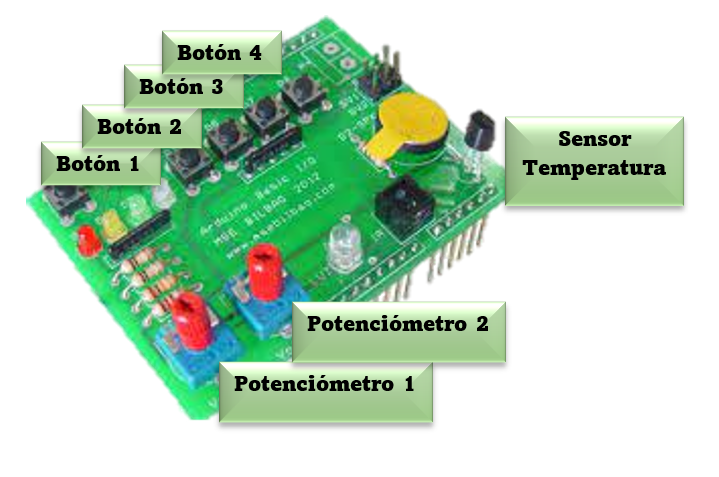
\includegraphics[width=0.7\textwidth]{shieldEtiquetado}
	\caption{Botones del shield de la placa maestro.}
\end{figure}
\FloatBarrier

\begin{figure}[!h]
	\centering
	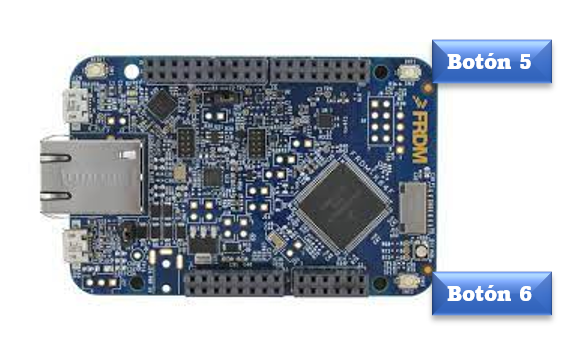
\includegraphics[width=0.7\textwidth]{botonesK64F}
	\caption{Botones utilizados de la placa K64F.}
\end{figure}
\FloatBarrier

\begin{description}
\item Para configurar la velocidad del motor A deberemos mover el potenciómetro 1 de la placa según la velocidad (sentido del giro) que le queramos asignar. Si lo giramos hacia la derecha completamente el motor recibirá el valor 255 y girará hacia la derecha, si por el contrario lo giramos hacia la izquierda recibirá el valor de 0 y girará en el sentido opuesto. En caso de que dejemos el potenciómetro en un rango medio de su giro, el motor recibirá el dígito 128 y dejara el motor parado.
\clearpage

\begin{figure}[!h]
 \centering
  \subfloat[Regulo potenciómetro 1]{
   \label{MUPoten1}
    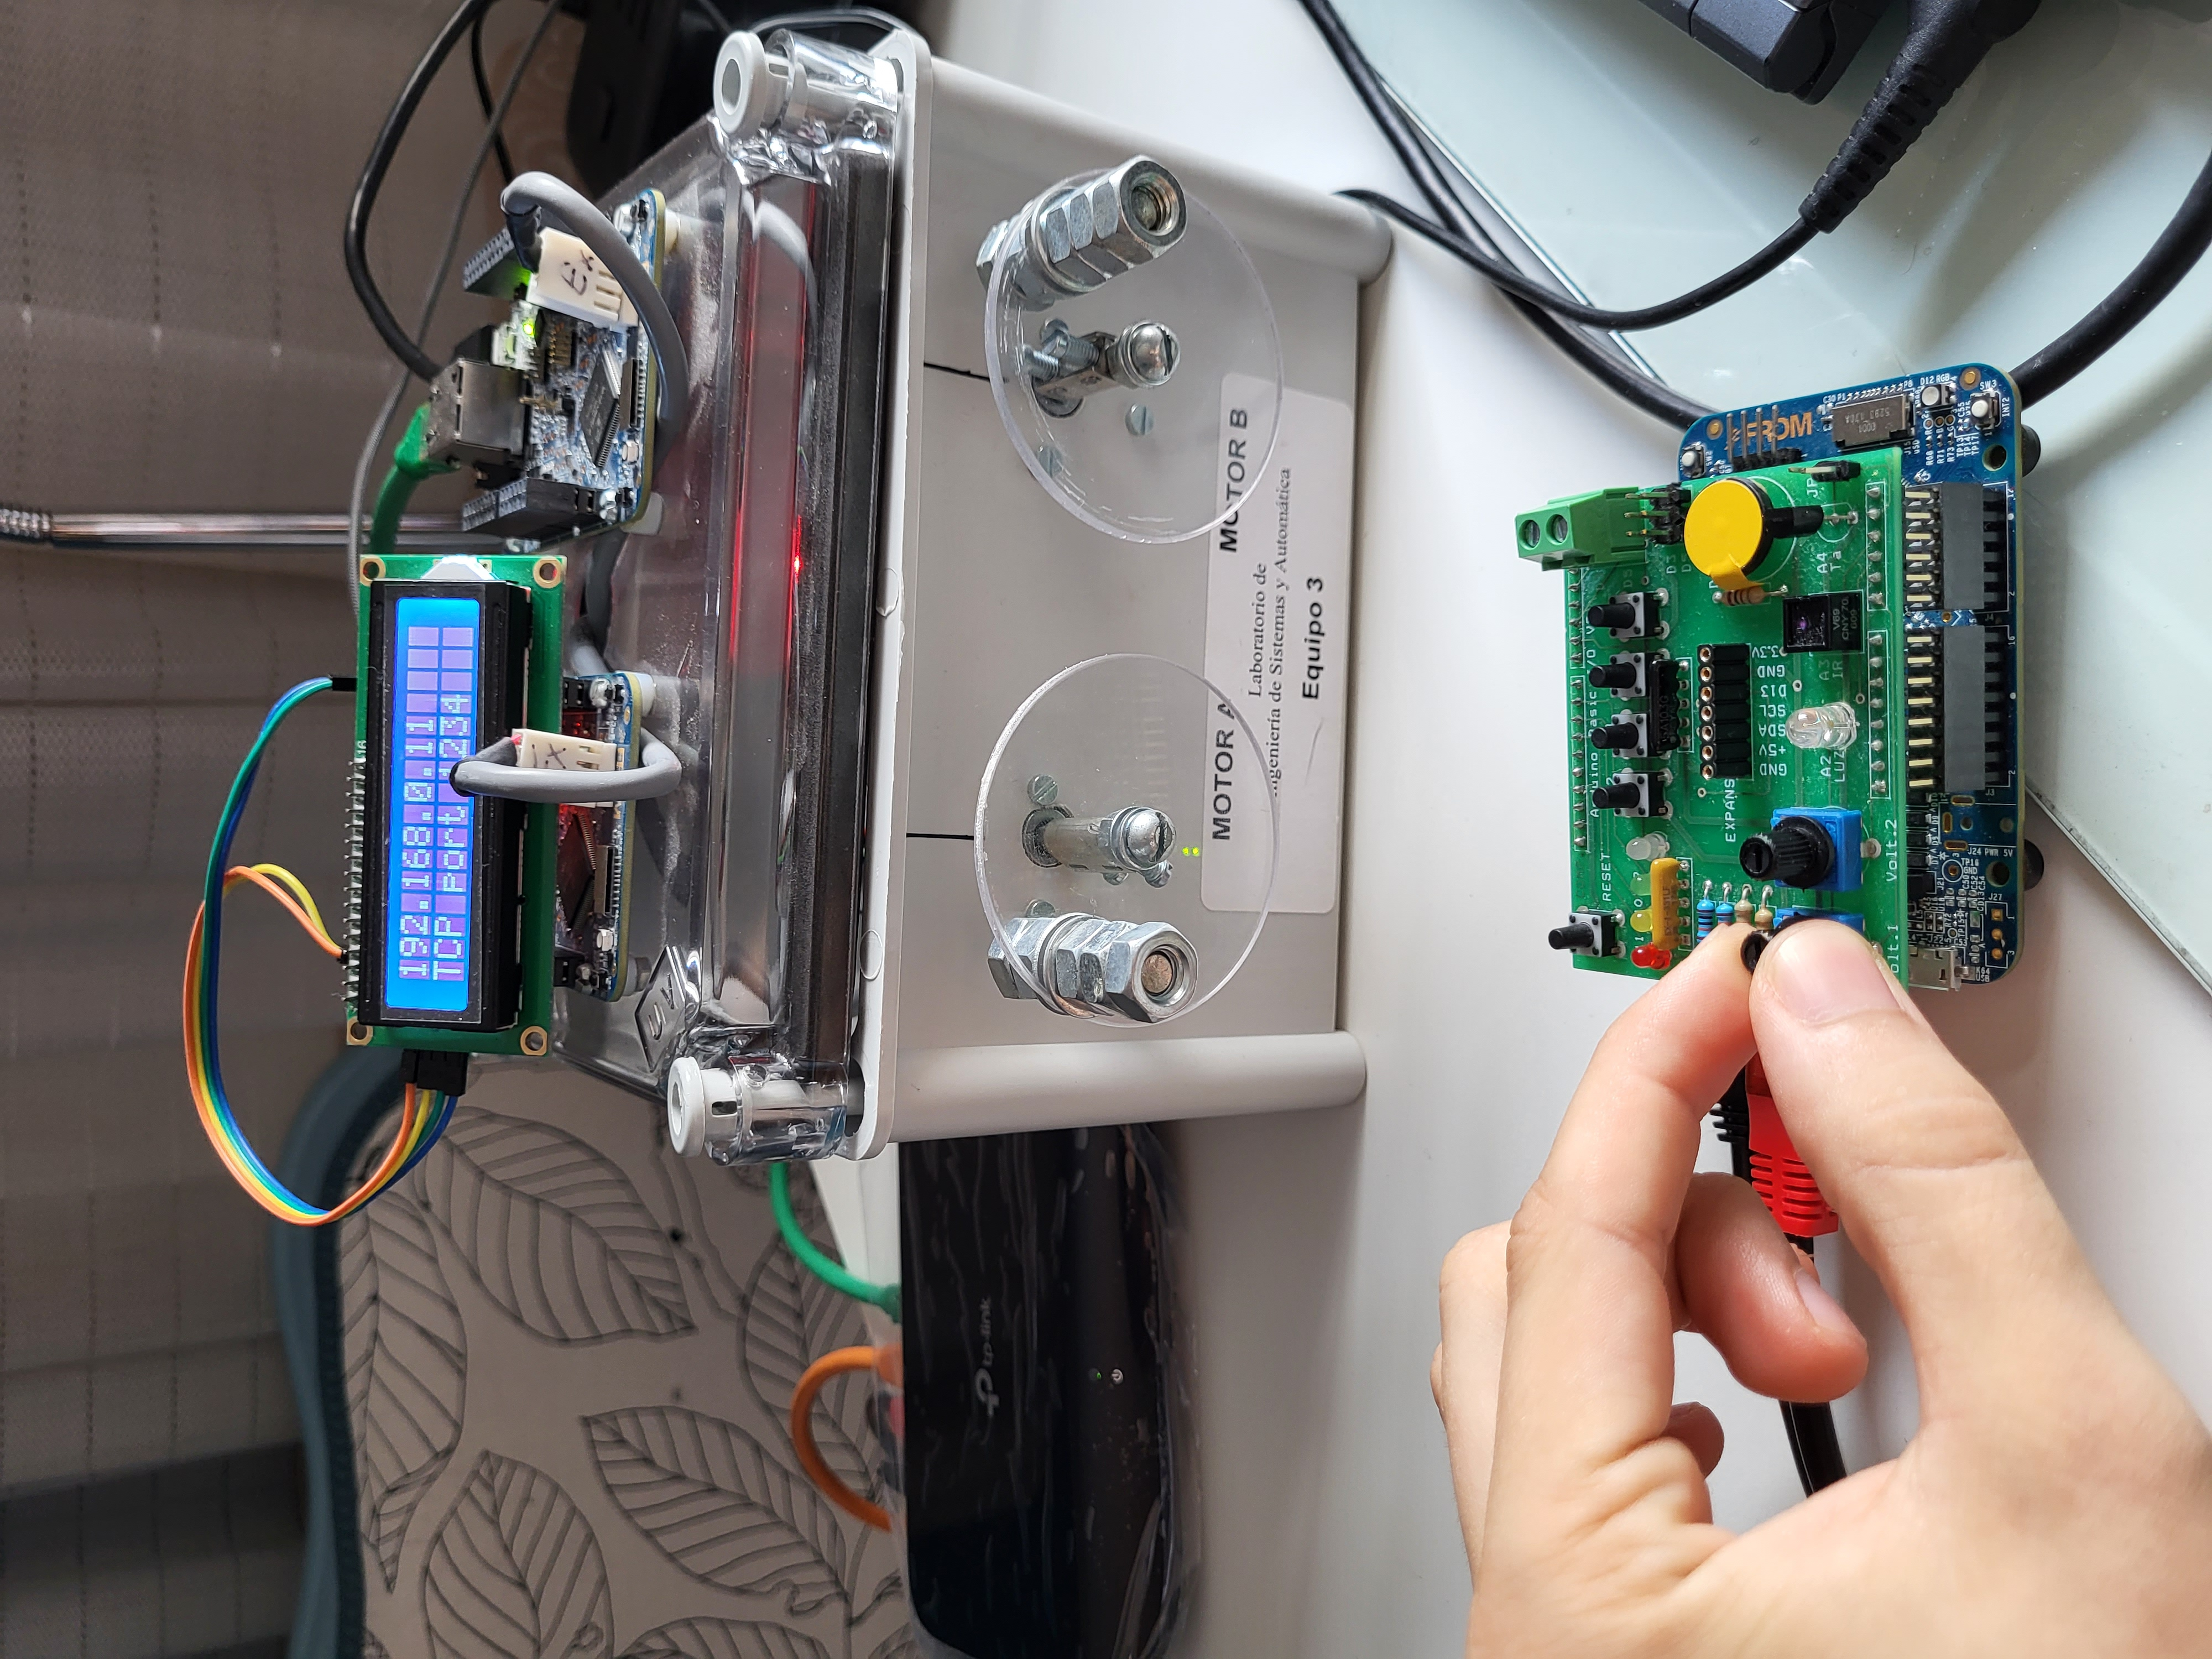
\includegraphics[angle=270,width=0.35\textwidth]{MUPoten1.jpg}}
  \subfloat[Pulso Botón 1]{
   \label{MUBoton1}
    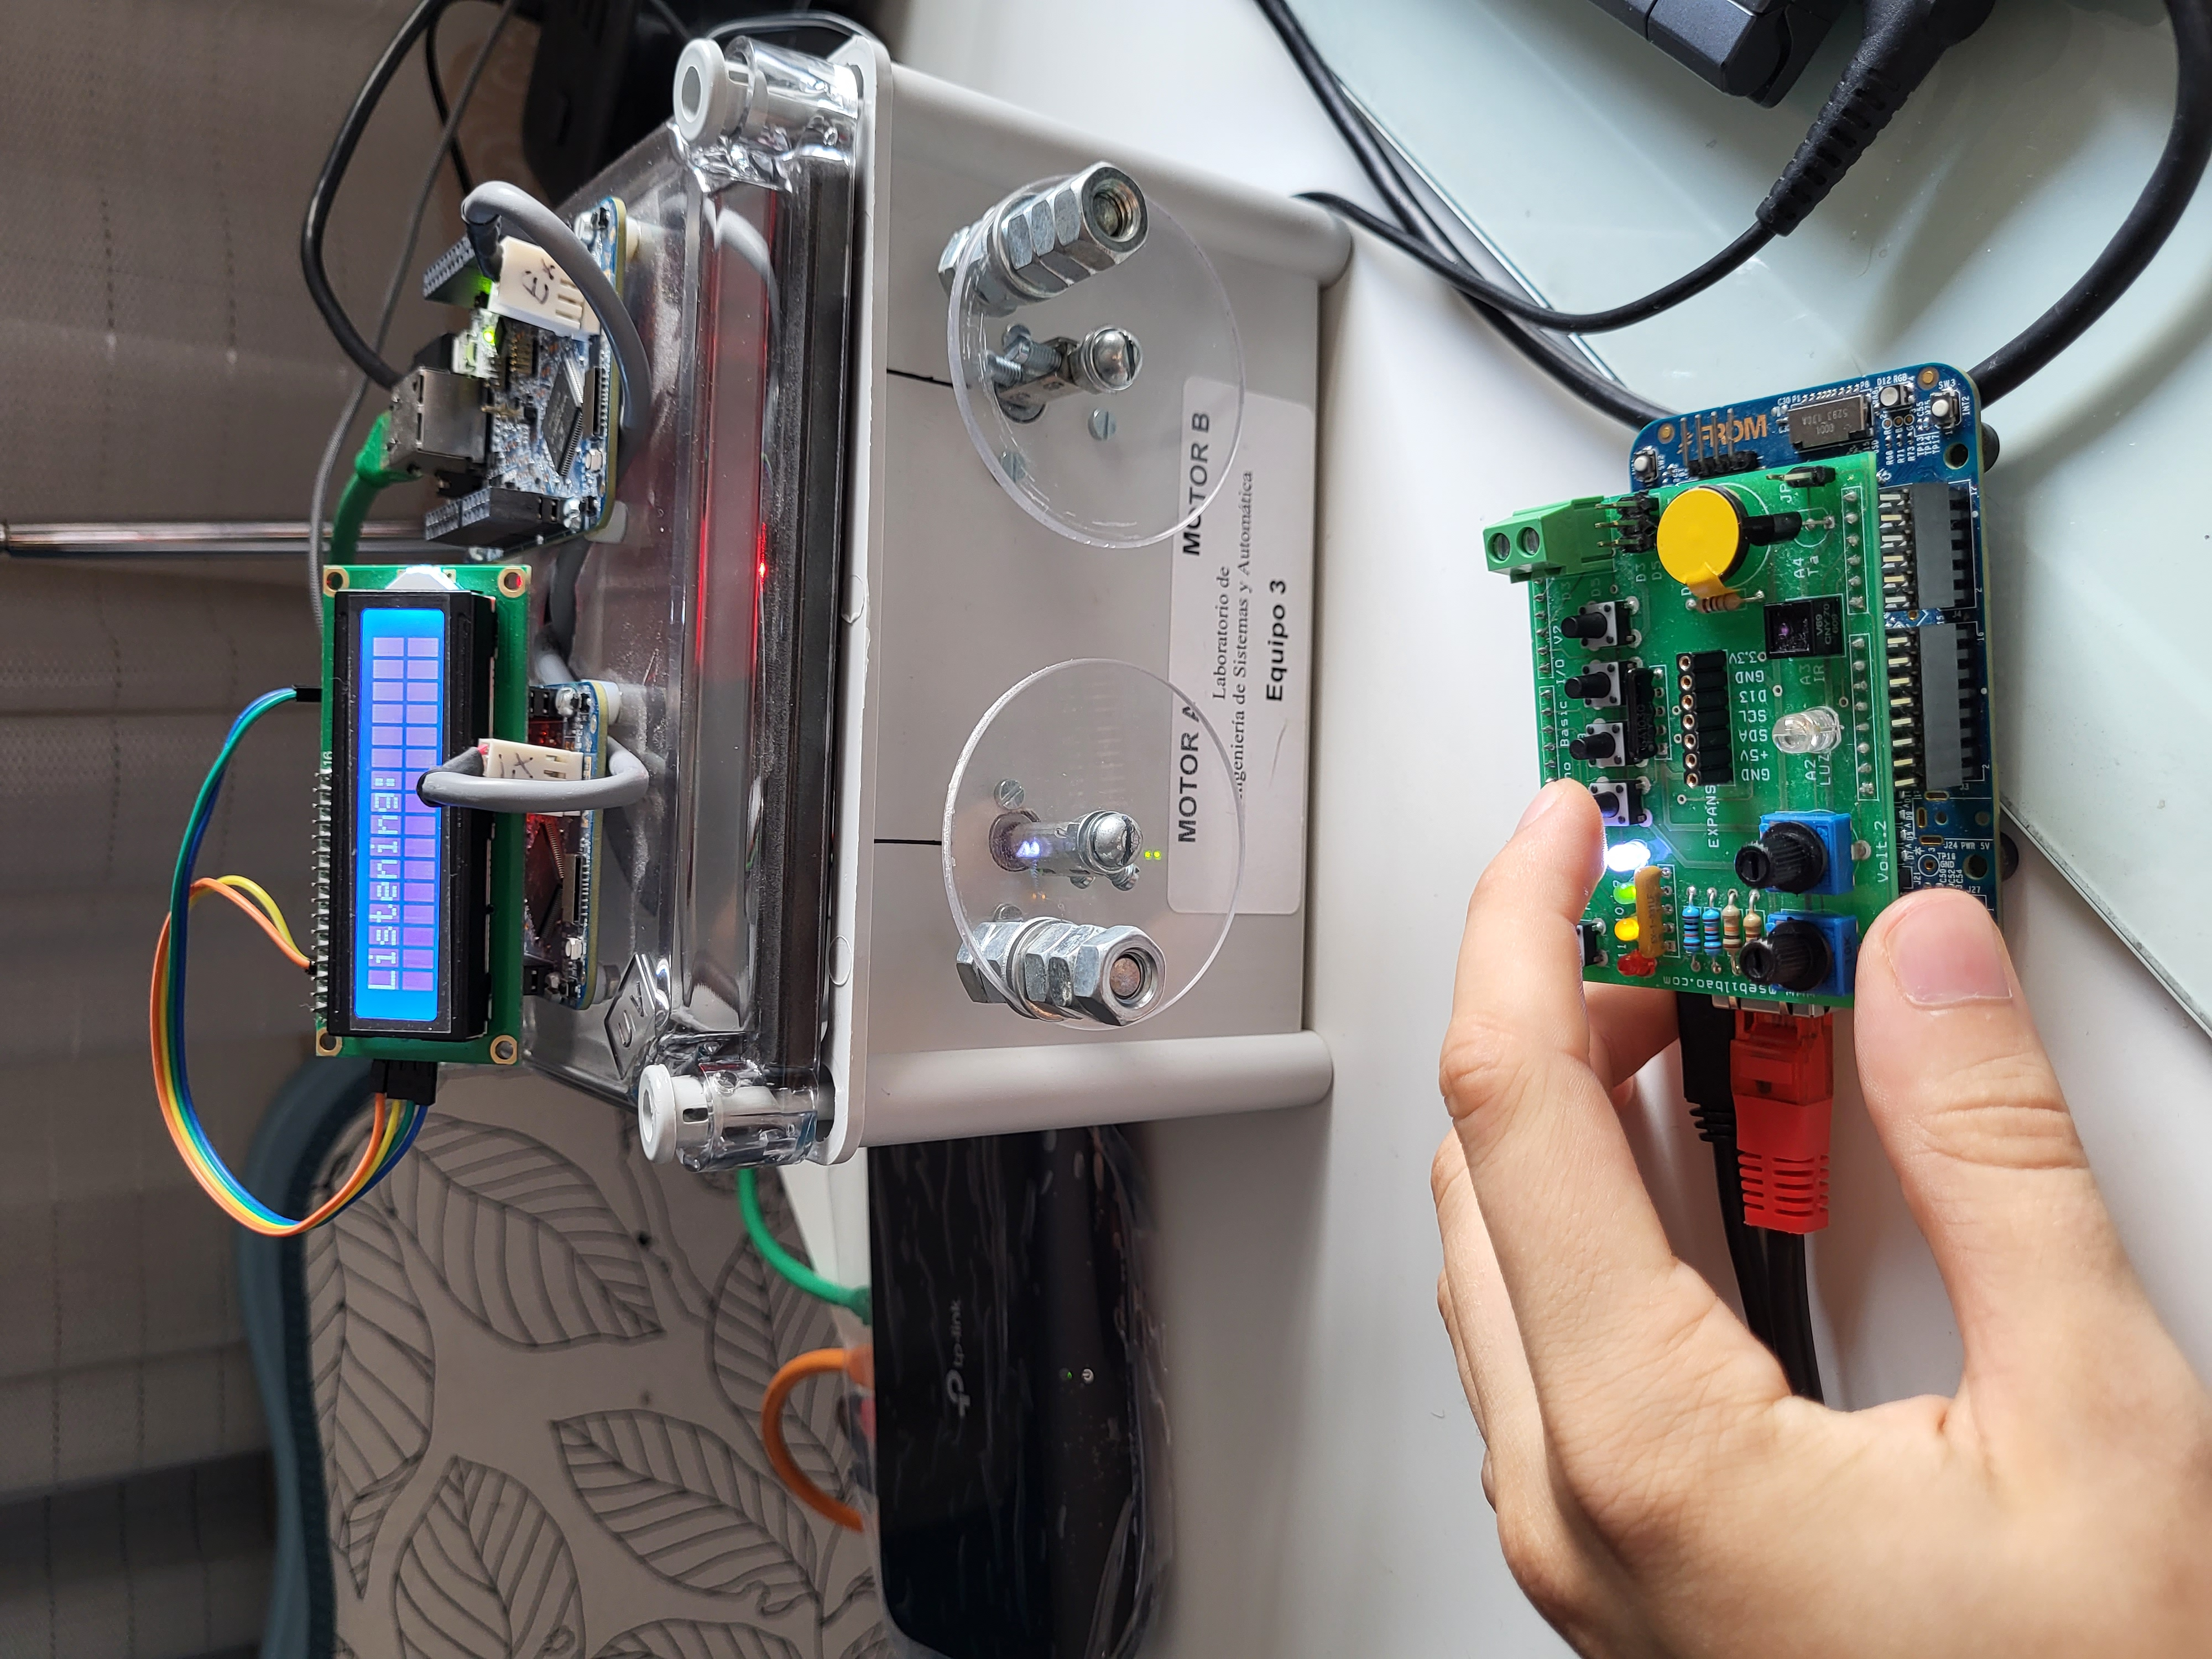
\includegraphics[angle=270,width=0.35\textwidth]{MUBoton1.jpg}}
 \caption{Establecer velocidad motor A.}
 \label{MU1}
\end{figure}



\item Lo mismo pasa con el potenciómetro 2 y el botón 2. En ambos casos, al pulsar el botón 1 o dos, recibiremos un \extranjerismo{feedback} en la placa esclavo mediante un mensaje en la pantalla que nos mostrará si se recibió el comando o no.

\begin{figure}[!h]
 \centering
  \subfloat[Regulo potenciómetro 2]{
   \label{MUPoten1}
    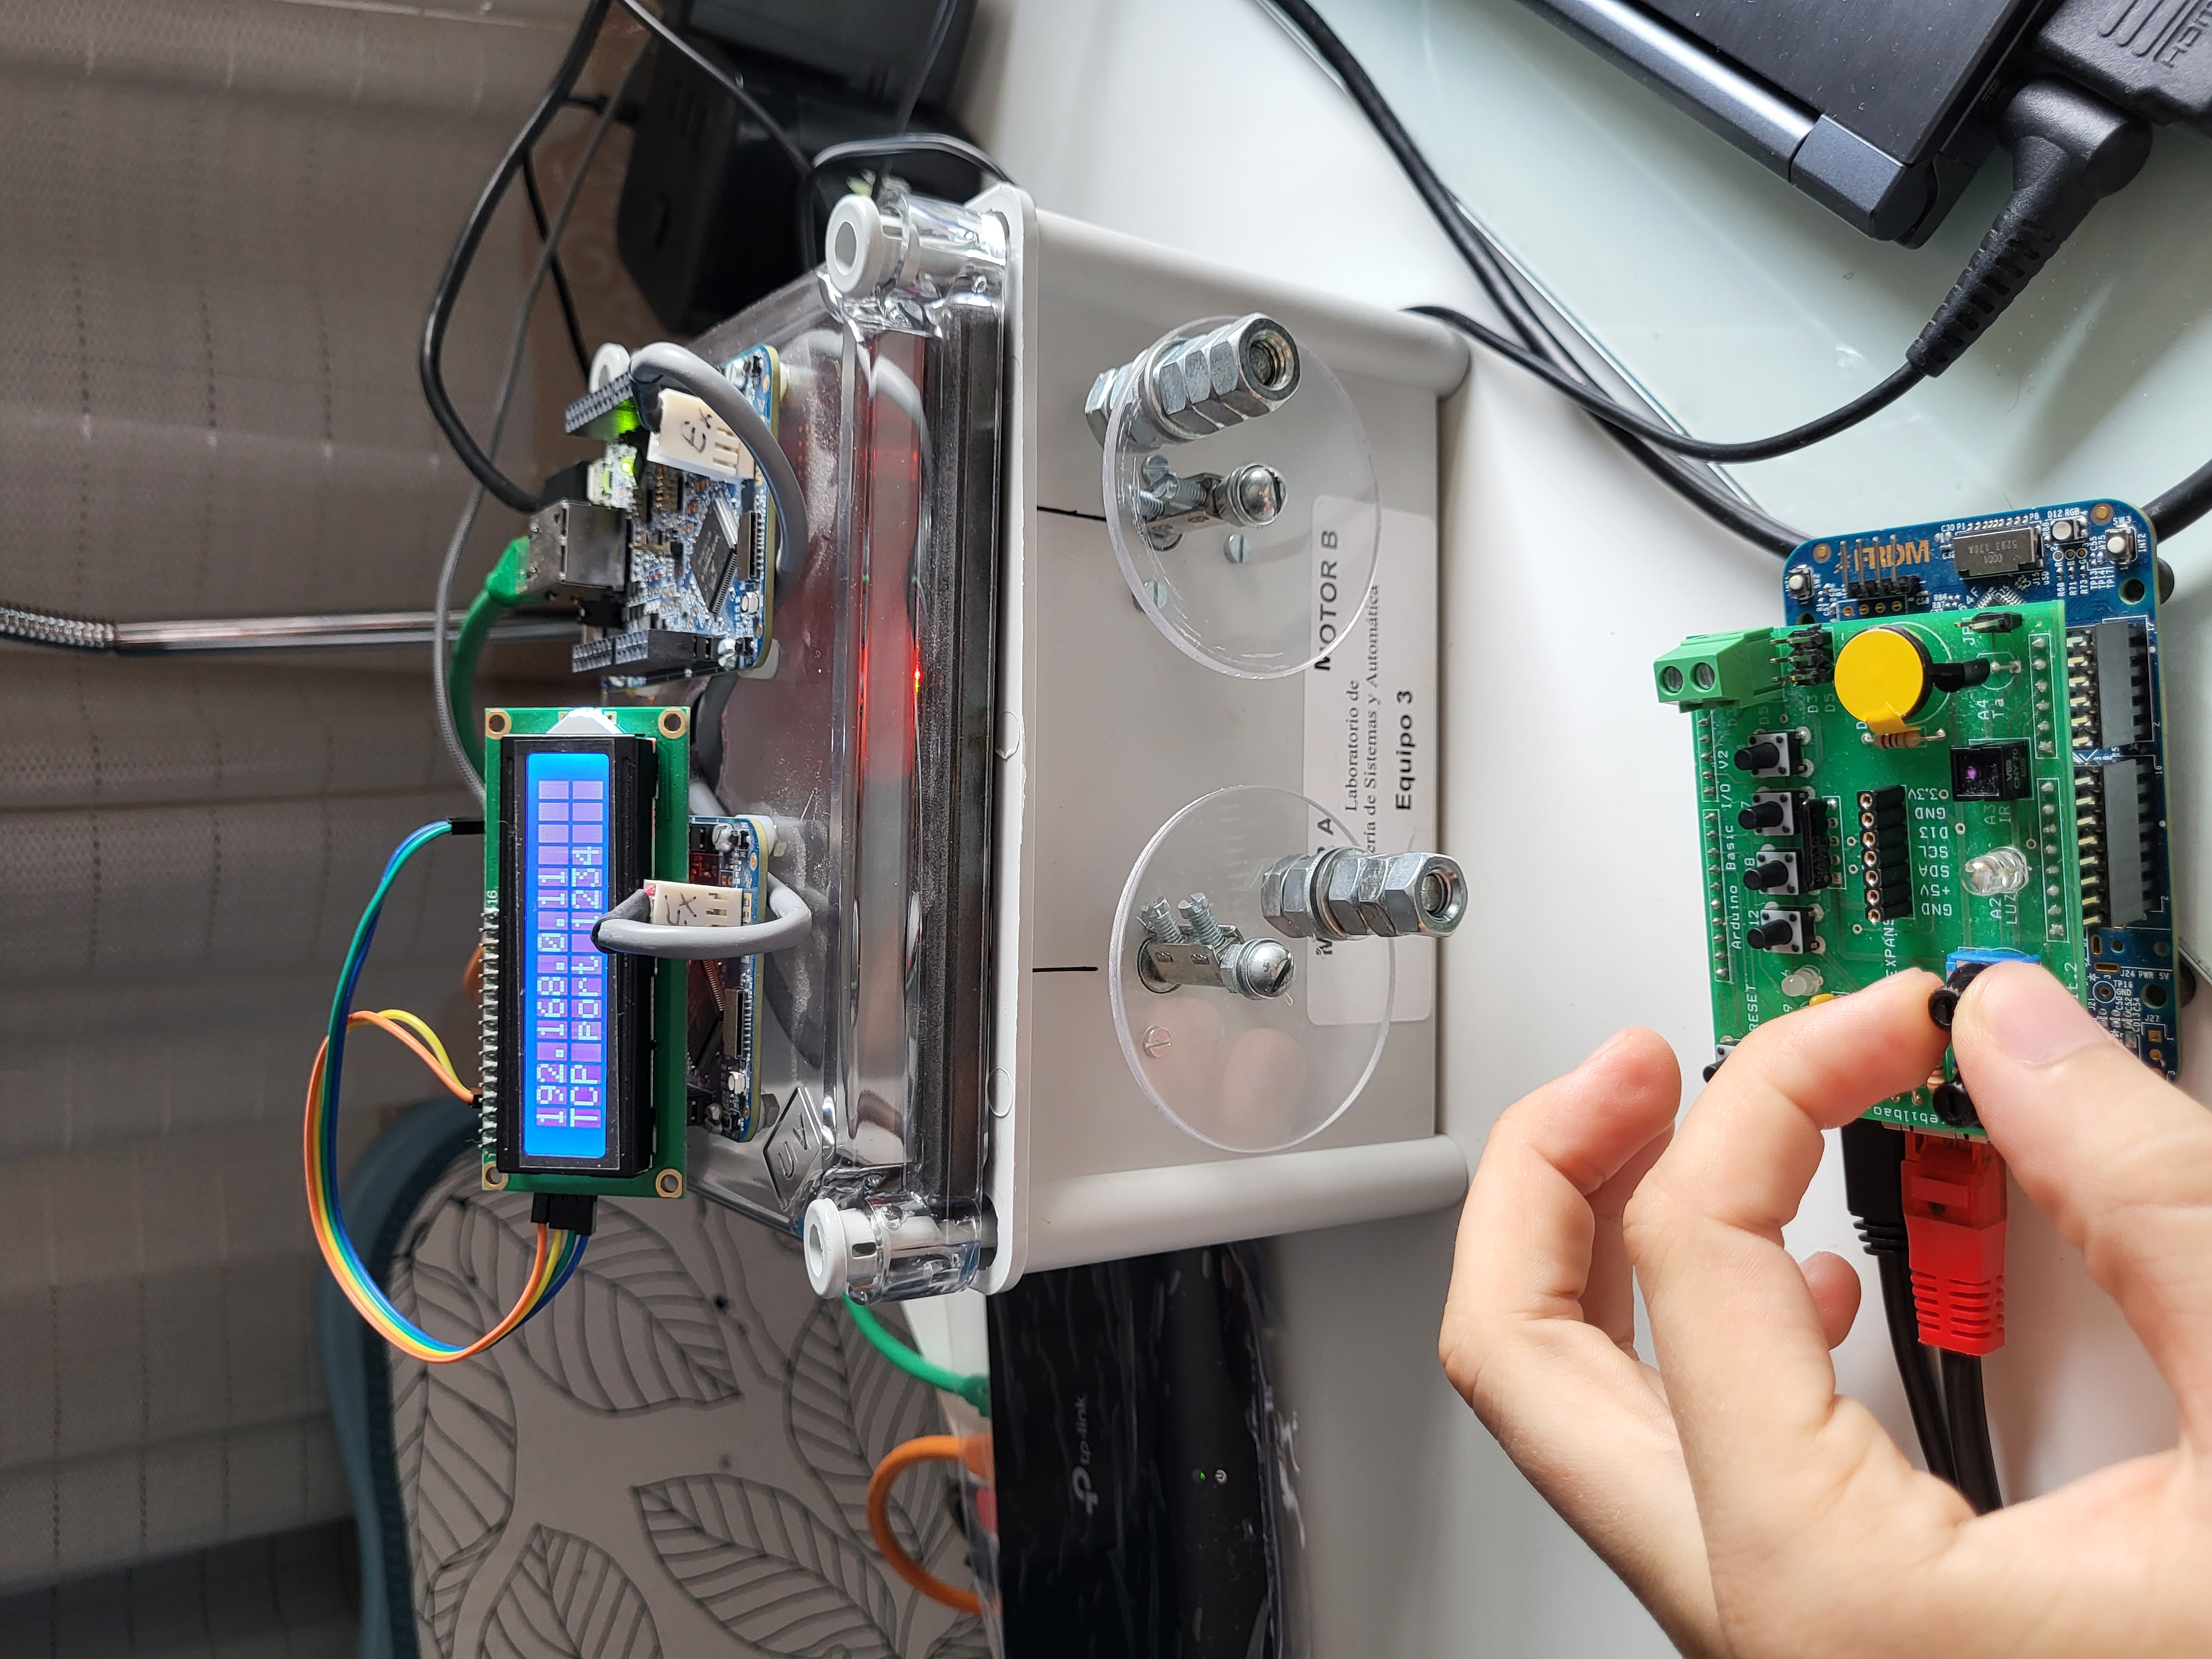
\includegraphics[angle=270,width=0.35\textwidth]{MUPoten2.jpg}}
  \subfloat[Pulso Botón 2]{
   \label{MUBoton1}
    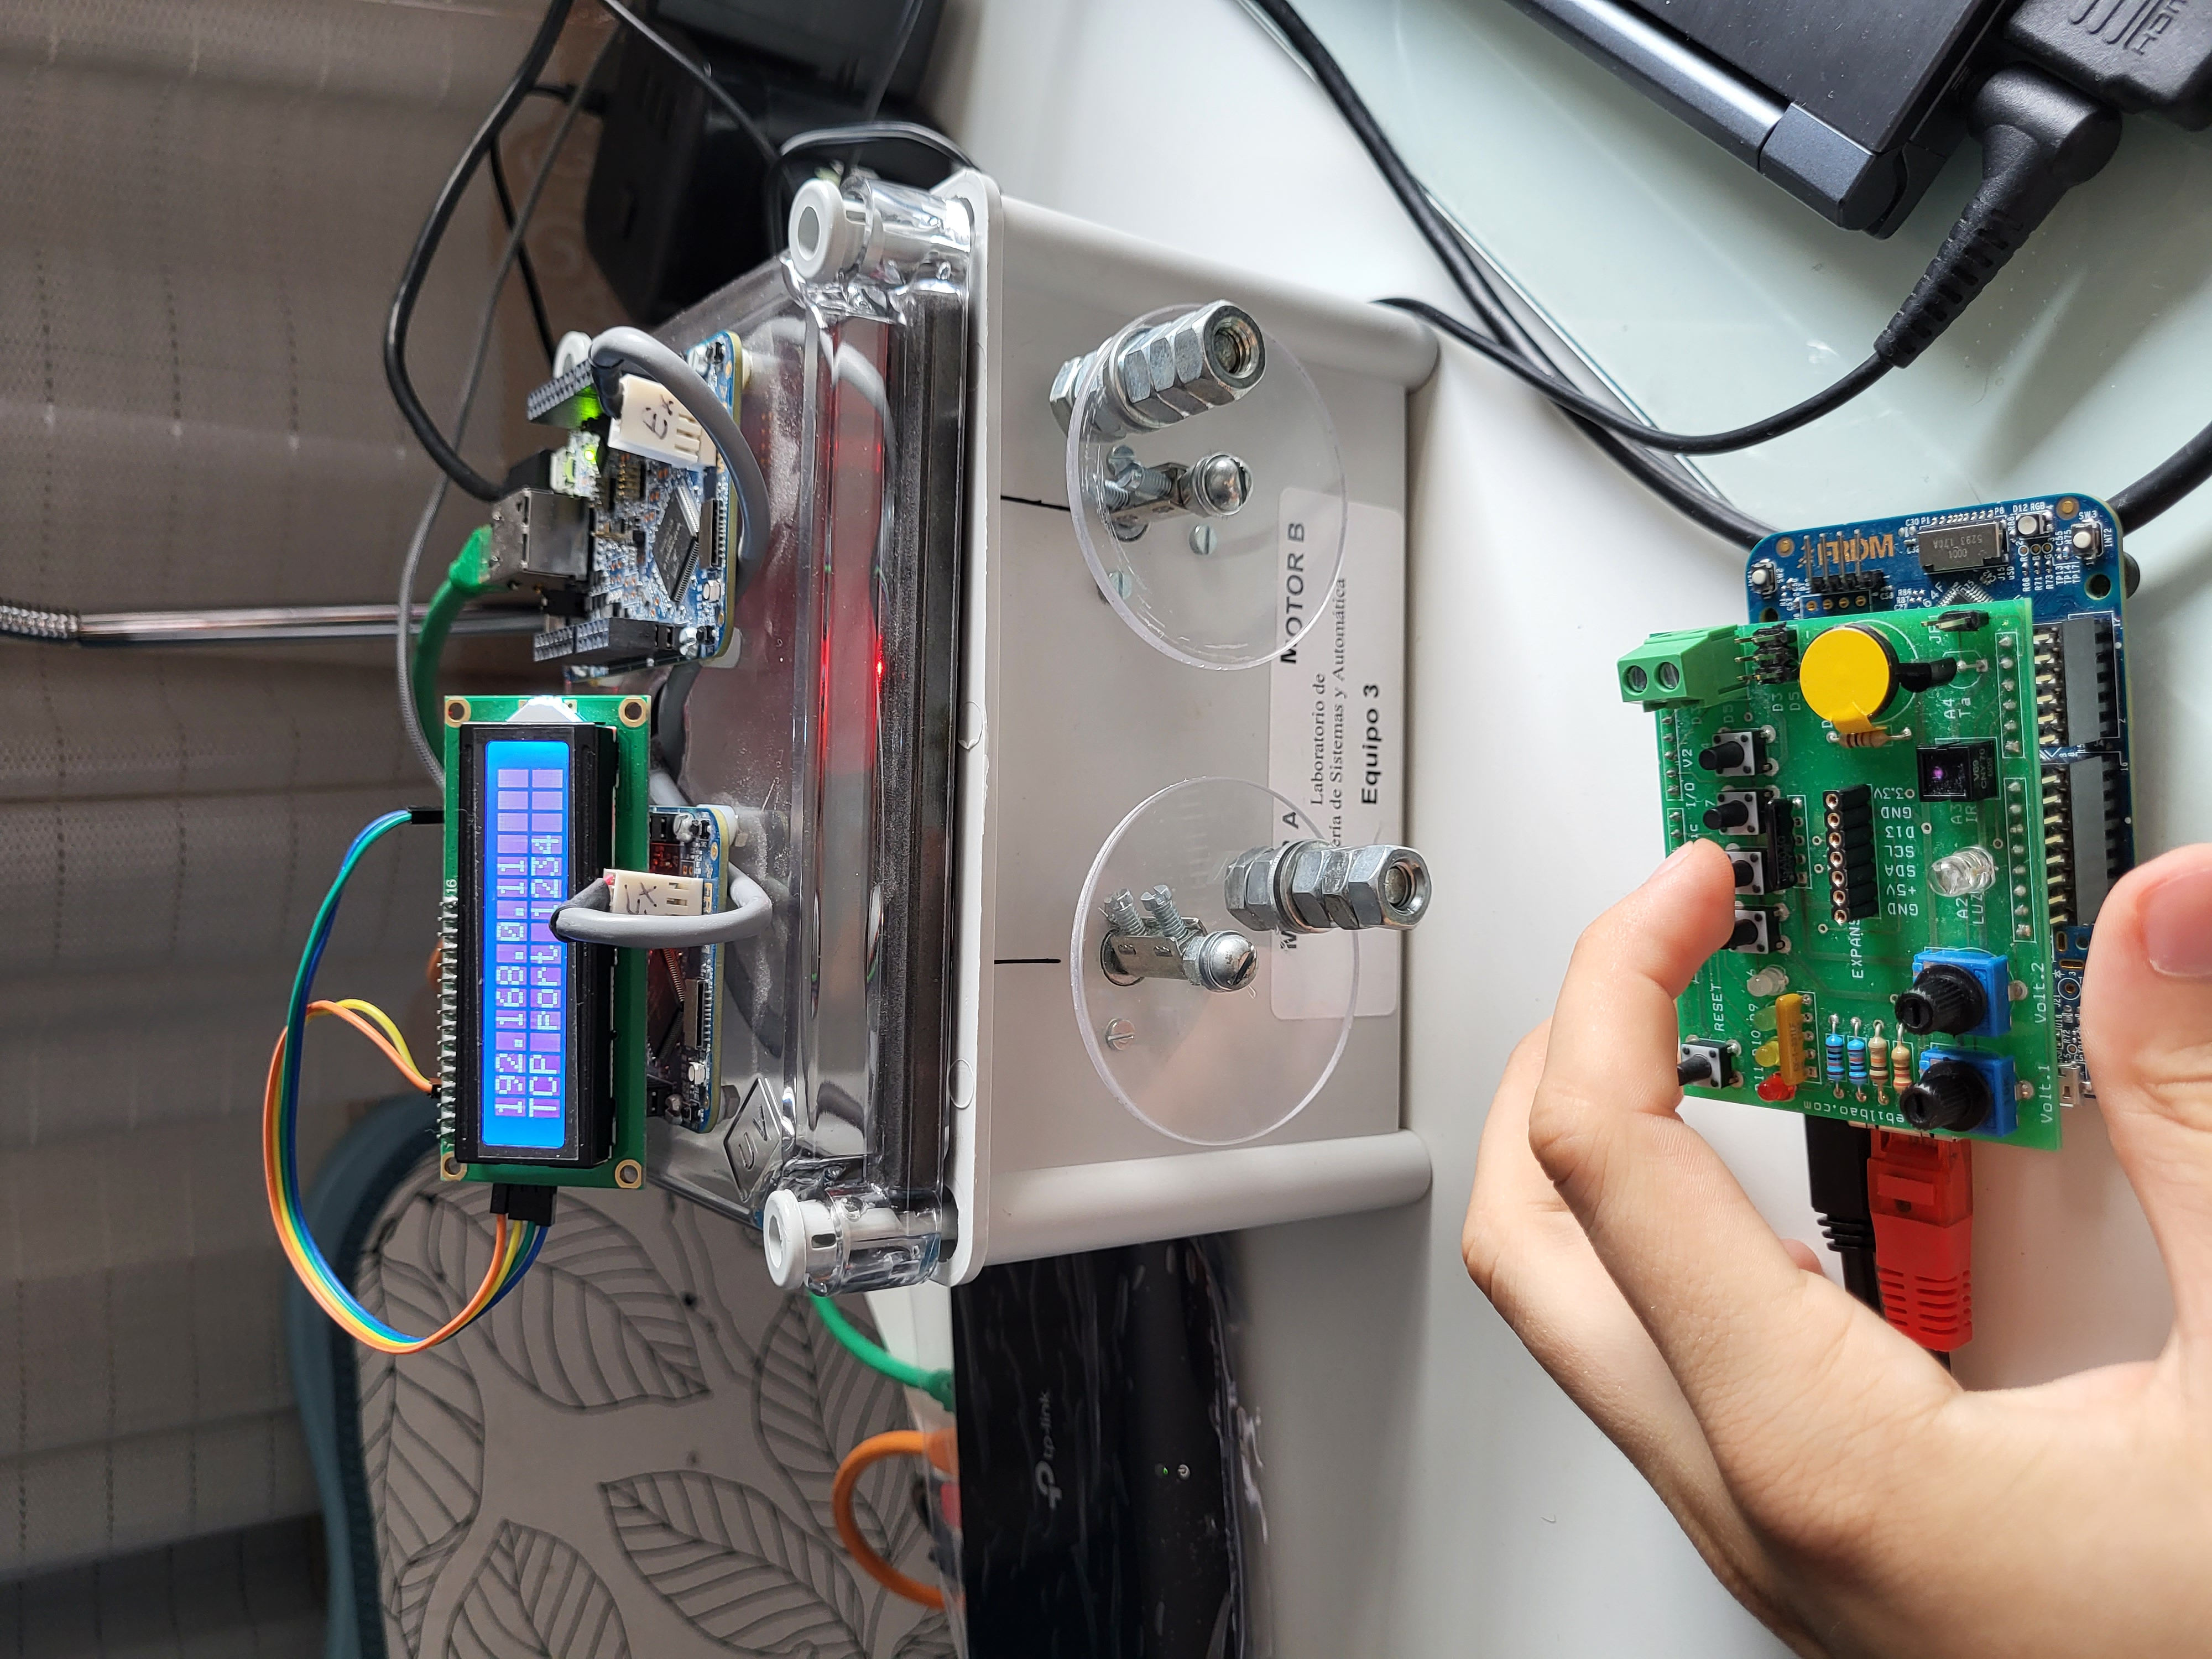
\includegraphics[angle=270,width=0.35\textwidth]{MUBoton2.jpg}}
 \caption{Establecer velocidad motor B.}
 \label{MU2}
\end{figure}

\item En caso de que queramos parar ambos motores utilizaremos el botón 3 a modo de parada de emergencia. 
\clearpage
\item El botón 4 envía a la placa maestro la temperatura ambiente. Esta temperatura se muestra en grados centígrados por la pantalla del esclavo. Mensaje que sale por pantalla: ``Temp actual: 23''.

\begin{figure}[!h]
	\centering
	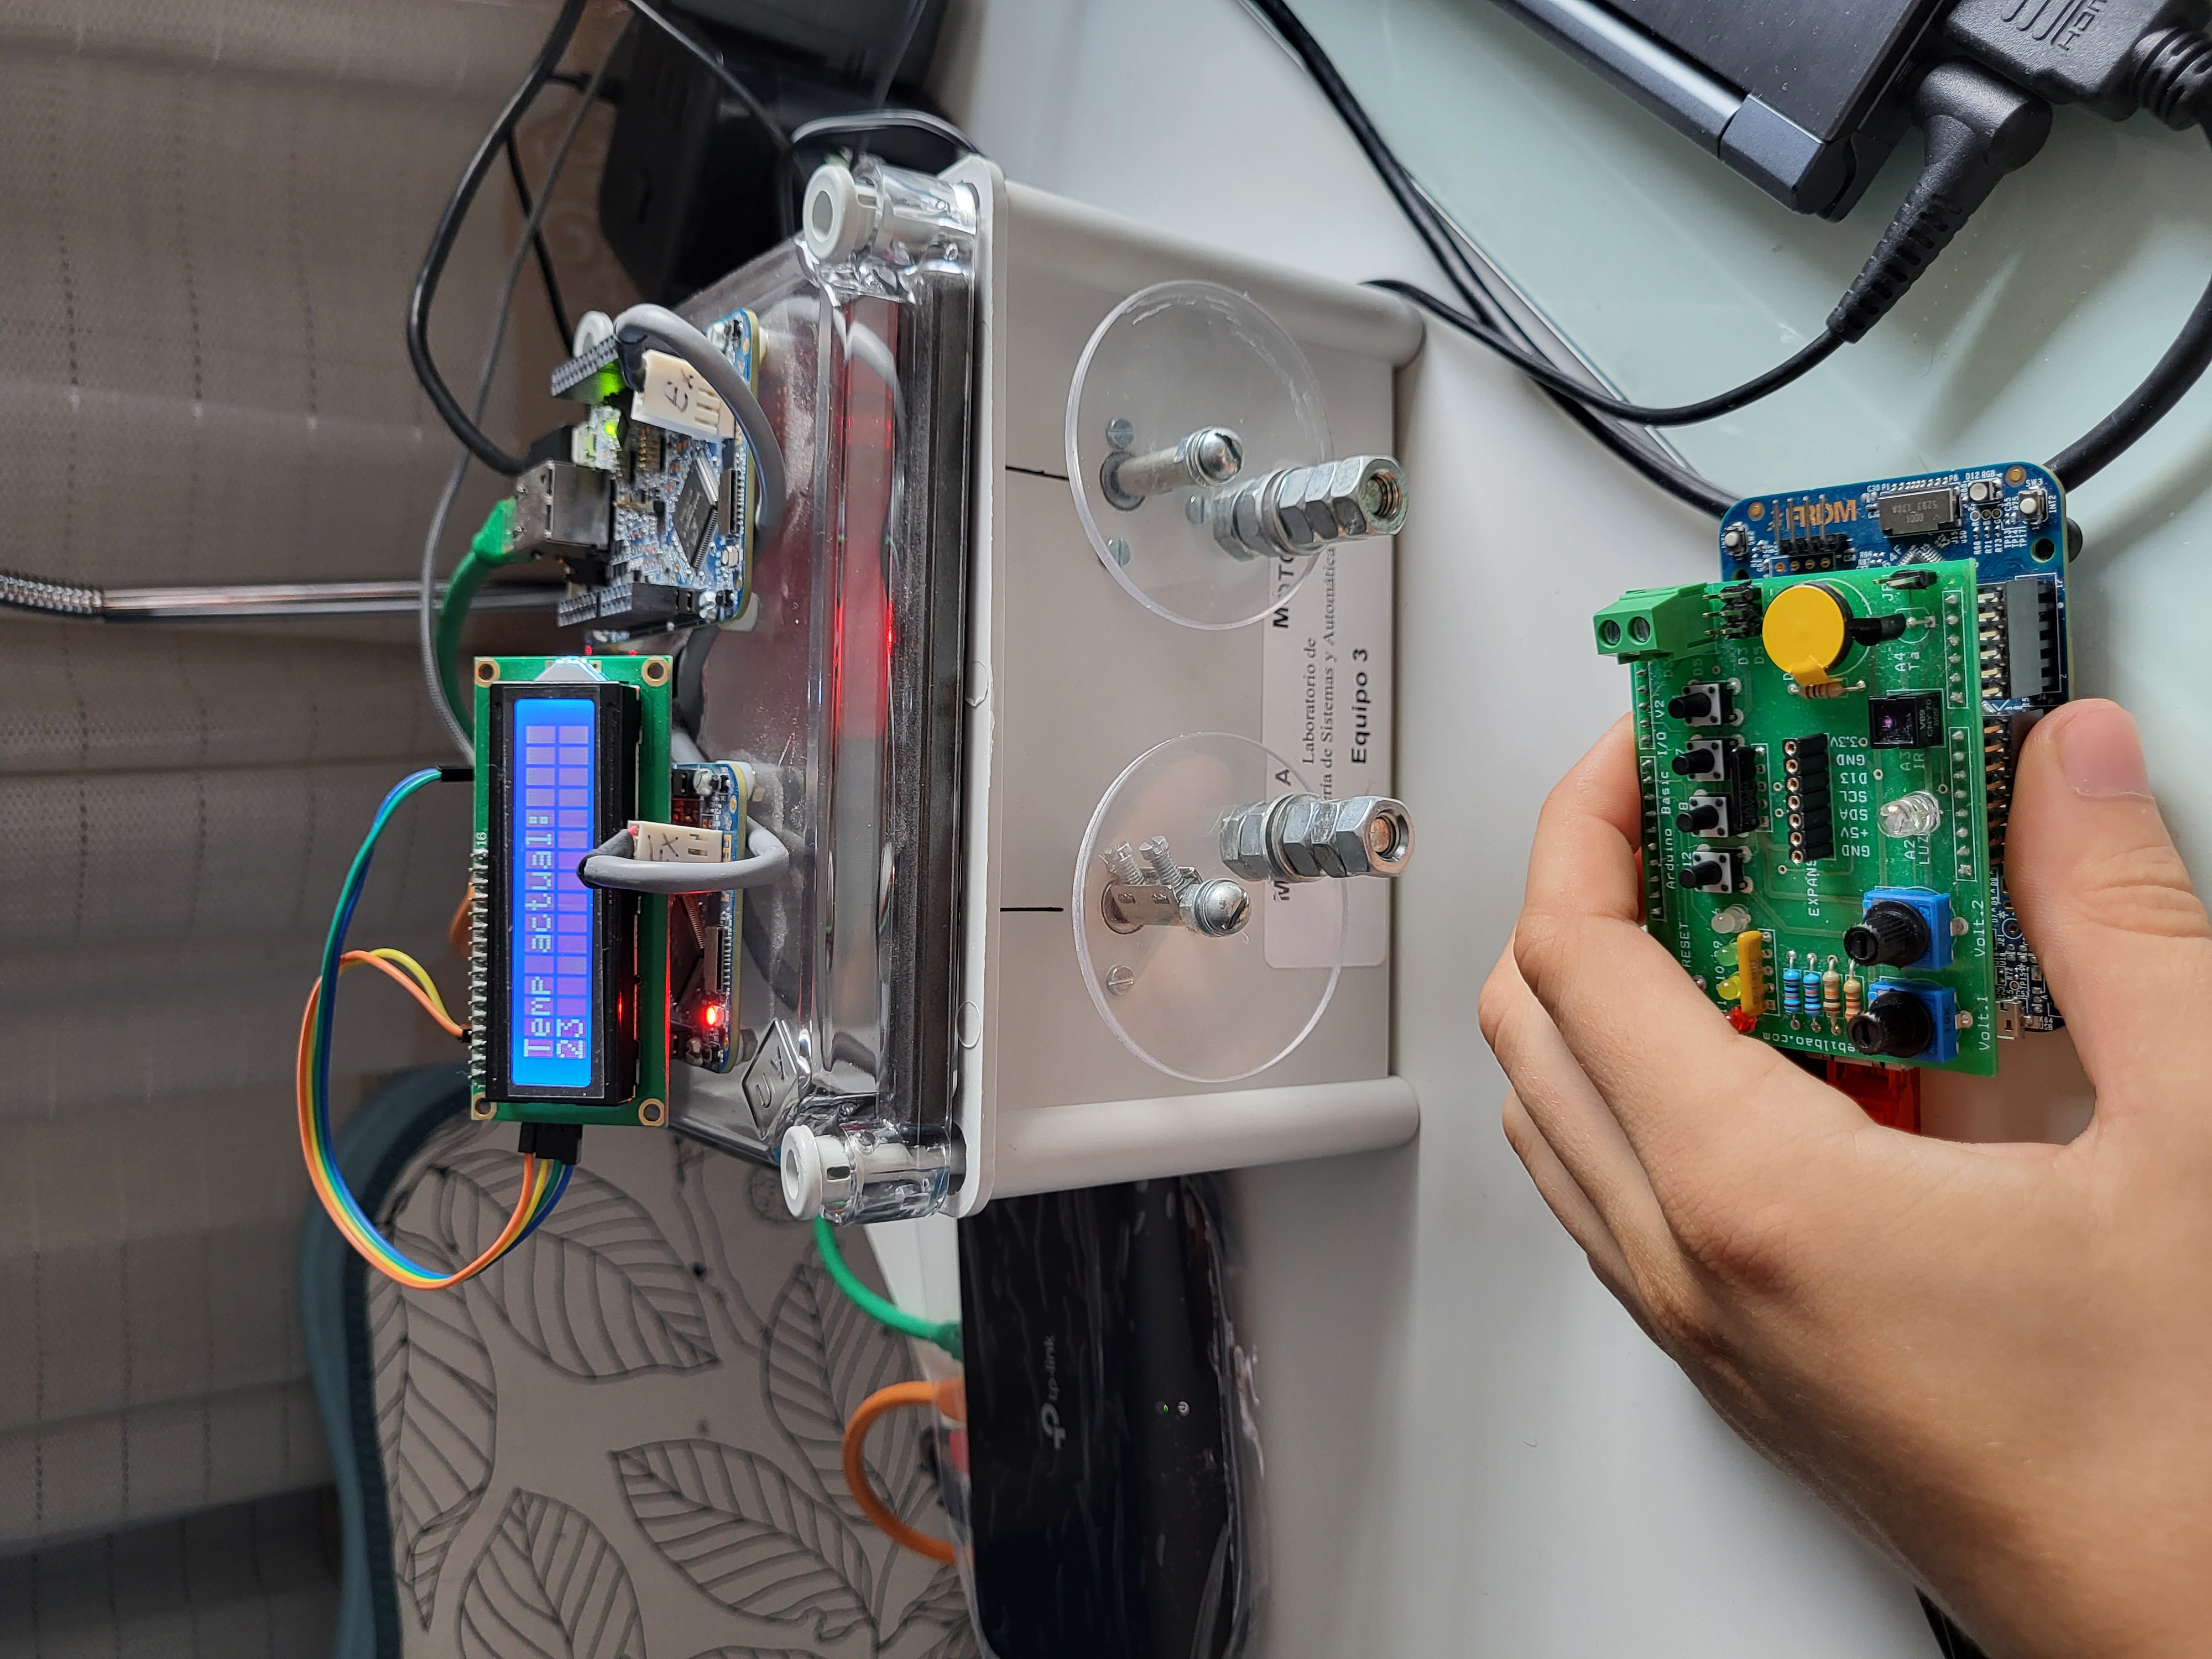
\includegraphics[angle=270,width=0.4\textwidth]{MUTemp.jpg}
	\caption{Se muestra la temperatura por pantalla.}
\end{figure}


\item Por último, los botones 5 y 6 muestran la velocidad de los motores A y B respectivamente, esta información se mostrará por la pantalla de la placa esclavo. Mensaje que muestra la pantalla: ``Vel motor 1: 255''.
\begin{figure}[!h]
 \centering
  \subfloat[Obtengo velocidad 1]{
   \label{MUPoten1}
    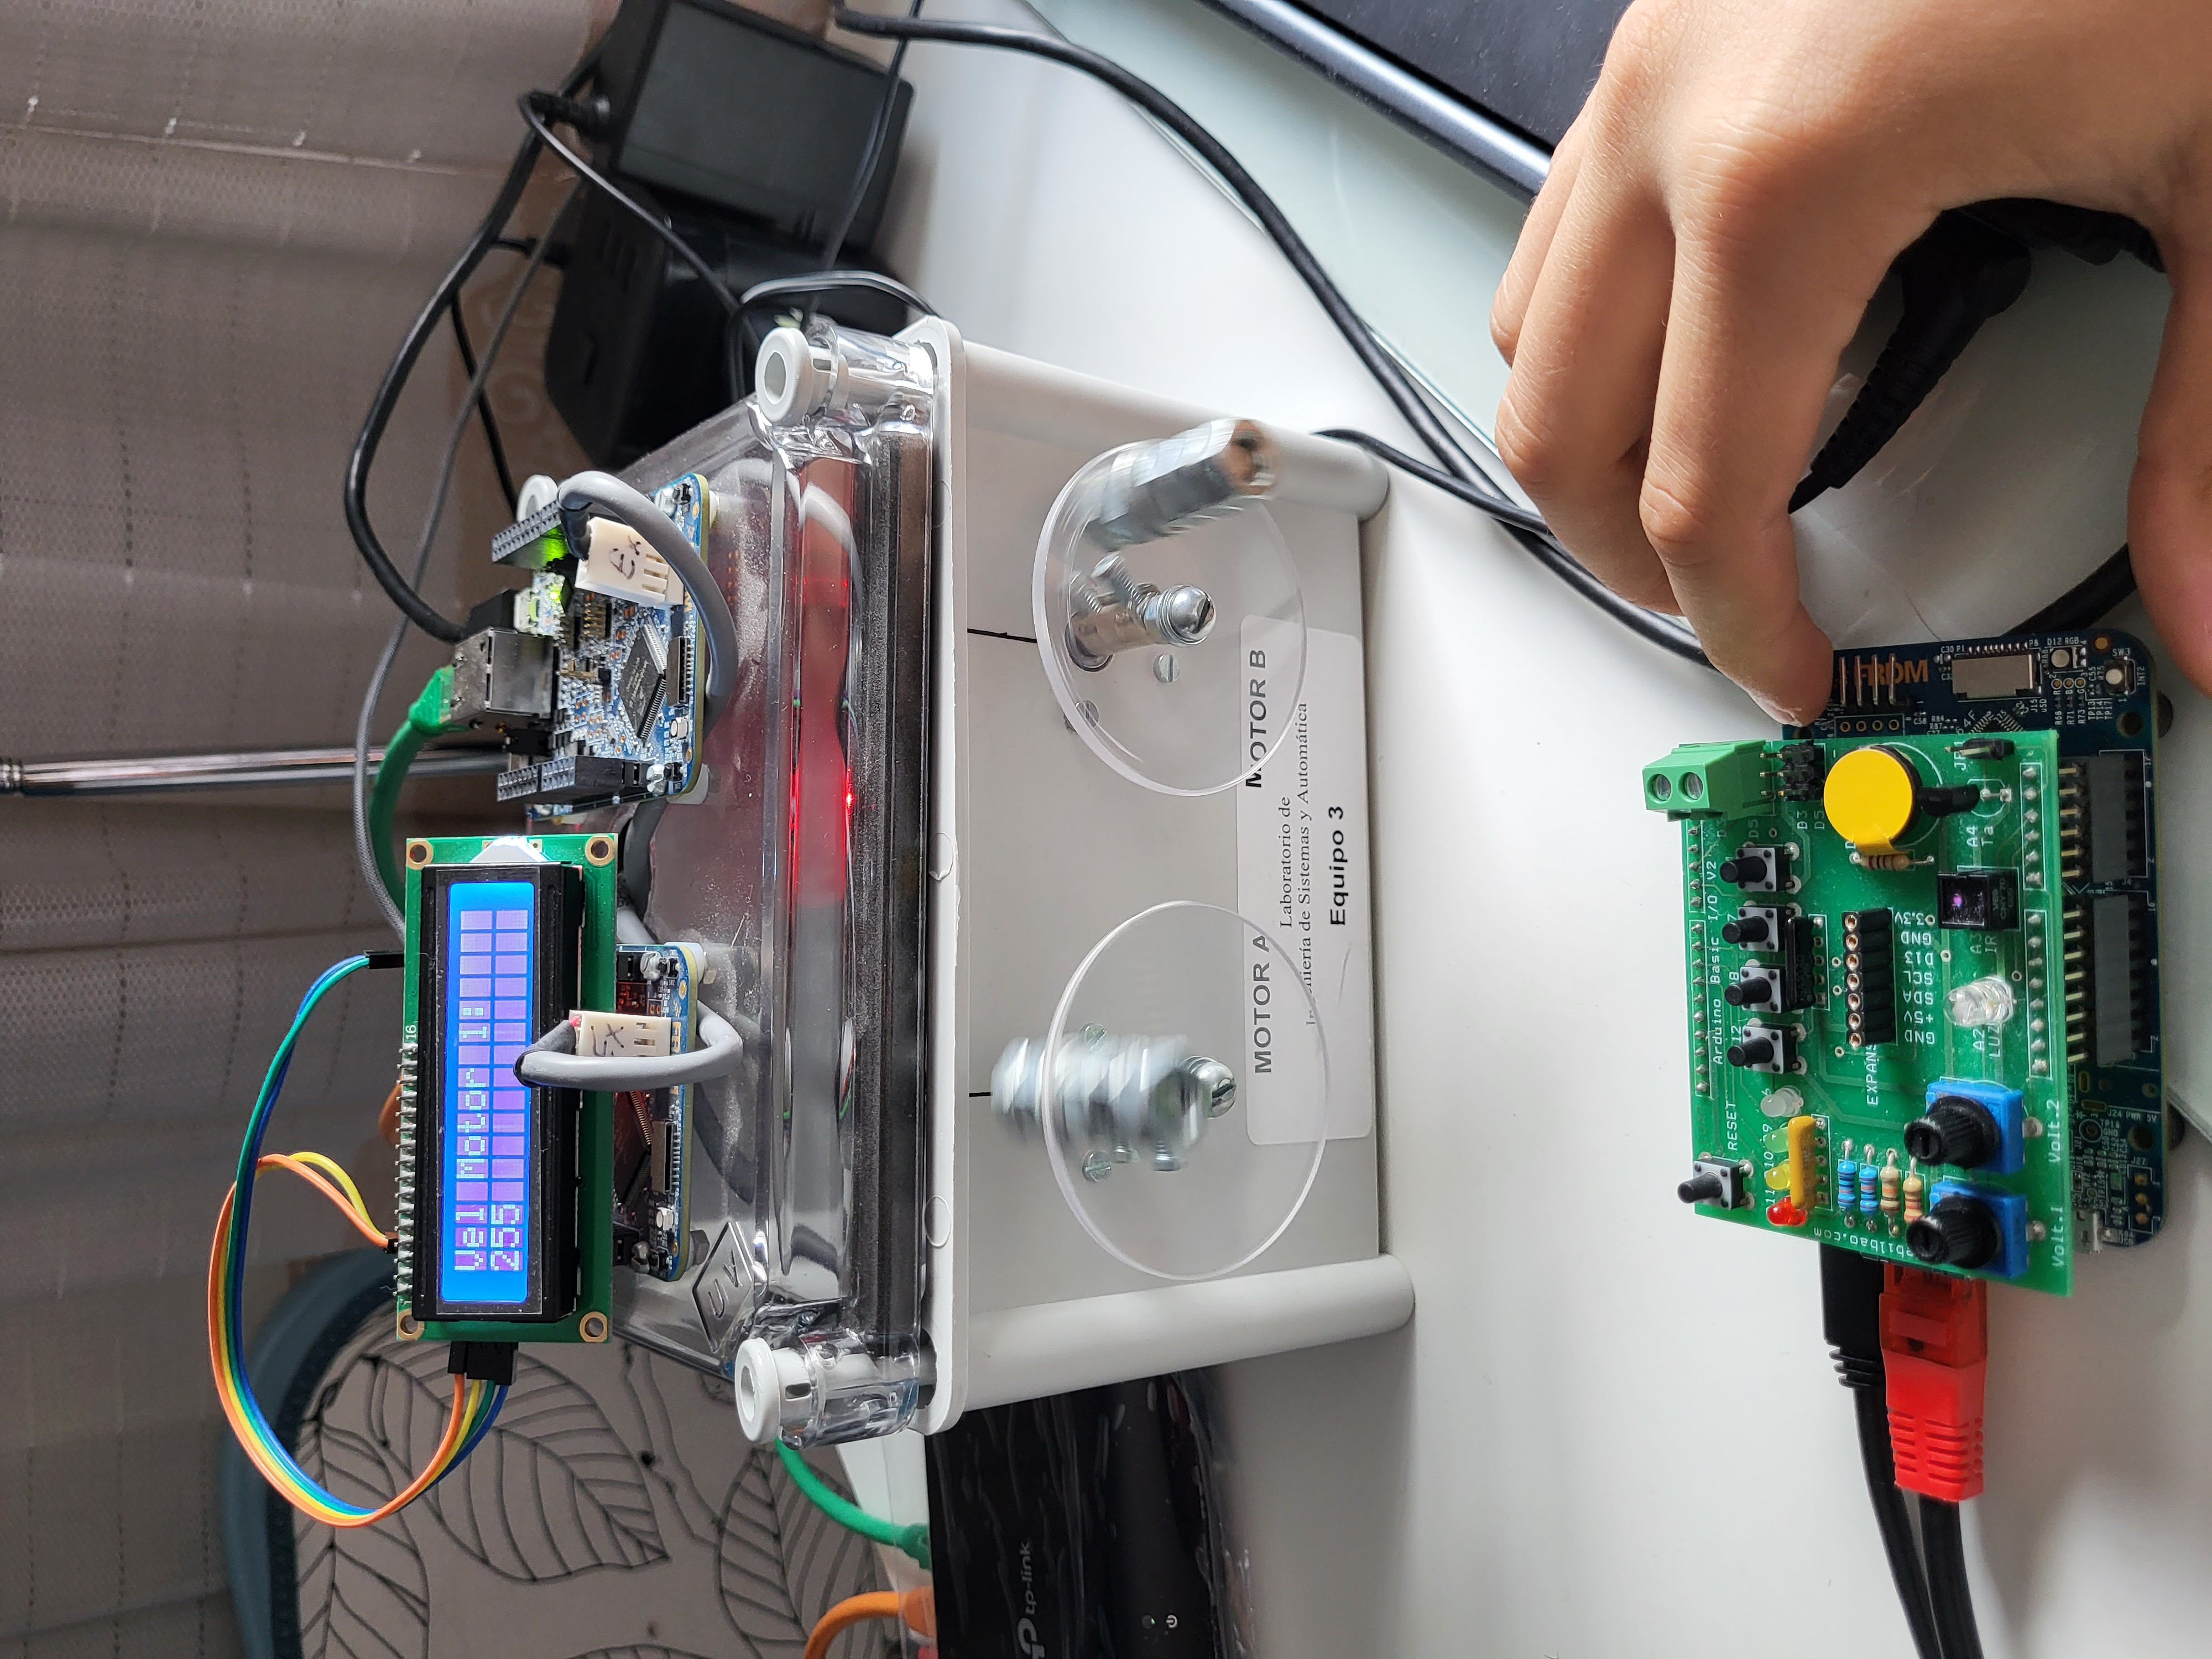
\includegraphics[angle=270,width=0.35\textwidth]{MUGvel1.jpg}}
  \subfloat[Obtengo velocidad 1]{
   \label{MUBoton1}
    \includegraphics[angle=270,width=0.35\textwidth]{MUGVel2.jpg}}
 \caption{Obtener velocidades de los motores.}
 \label{MU5}
\end{figure}

\end{description}


